\documentclass[a4paper]{article}

\usepackage{/c/tduong/home/tex/harvard/harvard}
%\VignetteIndexEntry{feature} 
\title{feature: R package}
\author{Tarn Duong}



\usepackage{/usr/lib/R/share/texmf/Sweave}
\begin{document}

\maketitle

\section{Introduction}

Feature significance is an extension of kernel density estimation, 
which is used to establish the statistical significance of 
features (like local modes). See \citeasnoun{chaudhuri99} for 1-dimensional data,
\citeasnoun{godtliebsen02} for  2-dimensional data and \citeasnoun{duong06}
for 3- and 4-dimensional data. \texttt{feature} is an R package for 
feature significance for 1- to 4-dimensional data.
  
There is one main function in this package, \texttt{featureSignif}. 
It has a range of options which allow
the user to compute and display kernel density estimates, significant gradient
and significant curvature regions. Significant gradient and/or
curvature regions often correspond to significant features. 
We cover the options here which a newcomer would most likely require. 
For the full range of options (e.g. varying
plotting colours), see \texttt{?featureSignif}.


\section{Examples}
The earthquake data set is contained in 
\texttt{feature}. It contains 510 observations, each consisting
of measurements of an earthquake beneath the Mt St Helens volcano.
The first is the longitude (in degrees, where a negative number
indicates west of the International Date Line), second  is
the latitude (in degrees, where a positive number indicates north of
the Equator) and the third  is the depth (in km, where a
negative number indicates below the Earth's surface).

For the univariate example, we take the log(--depth)
as our variable of interest. 
Figure \ref{fig:fs1} contains the kernel
density estimate with bandwidth 0.1 (in orange). Superimposed in green 
are the sections of this density estimate which have significant gradient
(i.e. significantly different from zero). The rug plot is 
the log(--depth) measurements.

\begin{figure}
\begin{center}
\begin{Schunk}
\begin{Sinput}
> library(feature)
\end{Sinput}
\begin{Soutput}
Loading required package: KernSmooth
KernSmooth 2.22 installed
Copyright M. P. Wand 1997
Loading required package: misc3d
Loading required package: rgl
feature 1.1-4 (2006)
\end{Soutput}
\begin{Sinput}
> data(earthquake)
> eq3 <- -log10(-earthquake[, 3])
> featureSignif(eq3, addData = TRUE, addSignifGradRegion = TRUE, 
+     xlab = "-log(-depth)", bw = 0.1)
\end{Sinput}
\end{Schunk}
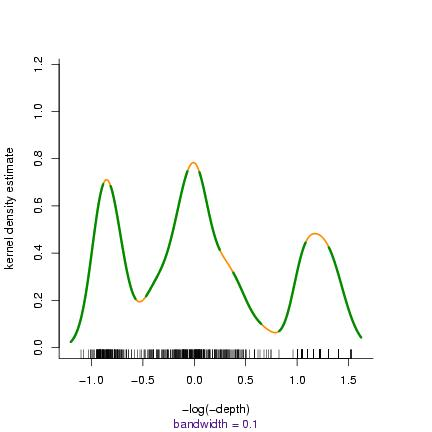
\includegraphics{feature-001}
\caption{Univariate data: significant gradient region with kernel density estimate}
\label{fig:fs1}
\end{center}
\end{figure}

Figure \ref{fig:fs2} contains the same kernel density estimate and 
significant gradient region plot along with the SiZer plot, see \citeasnoun{chaudhuri99}.
In the SiZer plot, blue indicates significantly increasing gradient,
red is significantly decreasing gradient, purple is non-significant gradient
and grey is data too sparse for reliable estimation. The horizontal black line
is for the bandwidth $0.1$.

\begin{figure}[!ht]
\begin{center}
\begin{Schunk}
\begin{Sinput}
> layout(matrix(1:2, nrow = 2))
> featureSignif(eq3, addSignifGradRegion = TRUE, xlab = "-log(-depth)", 
+     bw = 0.1)
> xlim <- par()$usr[1:2]
> featureSignif(eq3, plotSiZer = TRUE, xlab = "-log(-depth)", xlim = xlim)
> lines(c(-2, 2), c(0.1, 0.1))
> layout(1)
\end{Sinput}
\end{Schunk}
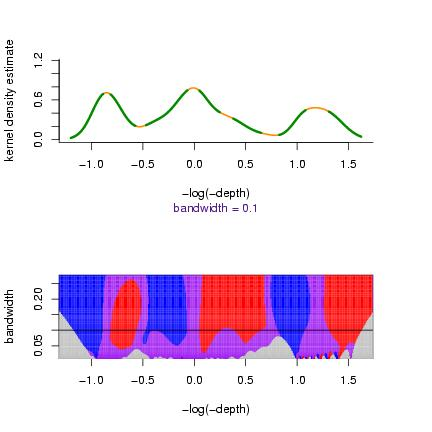
\includegraphics{feature-002}
\caption{Univariate data: significant gradient regions and SiZer plot}
\label{fig:fs2}
\end{center}
\end{figure}

\clearpage 
For bivariate data, we look at an Old Faithful geyser data set,
in the MASS library. The
horizontal axis is the waiting time (in minutes) between two eruptions, and
the vertical axis is the duration time (in minutes) of an eruption.
Figure \ref{fig:fs4} has a kernel density estimate with
bandwidth (4.5, 0.37),  with the significant gradient regions in green
and the significant curvature regions in blue superimposed.
\begin{figure}[!ht]
\begin{center}
\begin{Schunk}
\begin{Sinput}
> library(MASS)
> data(geyser)
> featureSignif(geyser, addSignifGradRegion = TRUE, addSignifCurvRegion = TRUE, 
+     bw = c(4.5, 0.37))
\end{Sinput}
\end{Schunk}
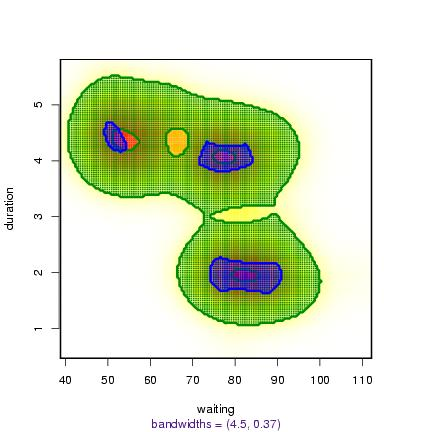
\includegraphics{feature-003}
\caption{Bivariate data: significant gradient and curvature regions}
\label{fig:fs4}
\end{center}
\end{figure}

A variation on plotting the significant regions is to plot the data points which
fall inside these regions in Figure \ref{fig:fs5}: 
significant gradient data points are in green,  
significant curvature data points are in blue.
\begin{figure}[!ht]
\begin{center}
\begin{Schunk}
\begin{Sinput}
> fs <- featureSignif(geyser, addSignifGradData = TRUE, addSignifCurvData = TRUE, 
+     bw = c(4.5, 0.37))
\end{Sinput}
\end{Schunk}
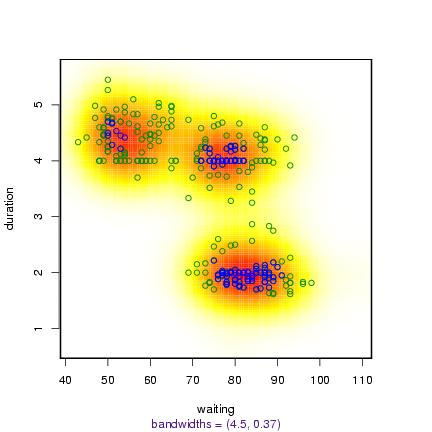
\includegraphics{feature-004}
\caption{Bivariate data: significant gradient and curvature data points}
\label{fig:fs5}
\end{center}
\end{figure}

\clearpage
Usually \texttt{featureSignif} 
returns invisbly to R but in this example, we assigned it to the variable 
\texttt{fs}.
\begin{Schunk}
\begin{Sinput}
> names(fs)
\end{Sinput}
\begin{Soutput}
[1] "x"        "bw"       "fhat"     "grad"     "curv"     "gradData" "curvData"
\end{Soutput}
\end{Schunk}
where x is the data, bw is the bandwidth, fhat\$est is the kernel density estimate
on the grid fhat\$x.grid, 
grad is the logical matrix indicating signficant gradient on a grid, 
curv is the logical matrix indicating signficant curvature on a grid,
gradData is the logical vector indicating signficant gradient data points and 
curvData is the logical vector indicating signficant curvature data points.
So the points with significant curvature are 
\begin{Schunk}
\begin{Sinput}
> fs$x[fs$curvData, ]
\end{Sinput}
\end{Schunk}
\begin{Schunk}
\begin{Soutput}
  waiting duration
1      80 4.016667
4      80 4.000000
5      75 4.000000
6      77 2.000000
9      77 2.033333
\end{Soutput}
\end{Schunk}
\vdots

\section{Functionality not documented in this vignette}

\texttt{feature} includes 
feature significance for 3- and 4-dimensional
data. However the displays in these dimensions rely on the rgl \cite{rgl}
engine which is not quite integrated with \texttt{Sweave} 
so we have excluded examples for the time being. See 
the example code in \texttt{?featureSignif}.   


These examples have used \texttt{feature} in its non-interactive
mode where the user supplies a particular value of the bandwidth. 
In its interactive mode, the user is able to choose a
bandwidth from a range of bandwidths and the significant features are
displayed in real-time.
Again it's not possible to illustrate this in this vignette,
see \texttt{?featureSignif}.   
 

\bibliographystyle{agsm}
%\bibliography{/c/tduong/home/research/references}

\begin{thebibliography}{xx}

\harvarditem{Adler \harvardand\ Murdoch}{2006}{rgl}
Adler, D. \harvardand\ Murdoch, D.  \harvardleft 2006\harvardright , {\em rgl:
  3D visualization device system (OpenGL)}.
\newblock R package version 0.67-2.

\harvarditem{Chaudhuri \harvardand\ Marron}{1999}{chaudhuri99}
Chaudhuri, P. \harvardand\ Marron, J.~S.  \harvardleft 1999\harvardright ,
  `Si{Z}er for exploration of structures in curves', {\em Journal of the
  American Statistical Association} {\bf 94},~807--823.

\harvarditem[Duong et~al.]{Duong, Cowling, Koch \harvardand\
  Wand}{2006}{duong06}
Duong, T., Cowling, A., Koch, I. \harvardand\ Wand, M.~P.  \harvardleft
  2006\harvardright , `Feature significance for multivariate kernel density
  estimation'.
\newblock Submitted.

\harvarditem[Godtliebsen et~al.]{Godtliebsen, Marron \harvardand\
  Chaudhuri}{2002}{godtliebsen02}
Godtliebsen, F., Marron, J.~S. \harvardand\ Chaudhuri, P.  \harvardleft
  2002\harvardright , `Significance in scale space for bivariate density
  estimation', {\em Journal of Computational and Graphical Statistics} {\bf
  11},~1--21.

\end{thebibliography}
 

\end{document}
